\subsection{Transformer Connector}\label{sec:transformer_experiments}
This section evaluates the transformer based connectors described in Section \ref{sec:transformer_methodology}. All transformer variants share the same inference pipeline as the XGBoost connector: the model outputs a merge probability for each tracklet pair, which is converted to a distance ($d=1-p$) and fed into hierarchical agglomerative clustering with average linkage. This allows a direct comparison between approaches, since only the pairwise scoring model differs. Three transformer architectures are evaluated (Siamese CLS, Cross-Attention, and Hybrid), alongside a simple MLP baseline that operates exclusively on handcrafted pairwise features.


\subsubsection{The Role of Pairwise Features}\label{sec:pairwise_ablation}
A natural assumption when applying transformers to the tracklet merging task is that the self-attention mechanism should be able to learn the relationships between two tracklet sequences directly from the per-frame features, without requiring handcrafted pairwise features such as ReID cosine similarity or temporal gap. If this assumption holds, the transformer would discover these relationships by comparing the raw frame sequences, making the explicit pairwise features redundant.

\

To test this assumption, we train the Siamese CLS architecture in two configurations: with and without the 12 pairwise features appended to the classification head. When pairwise features are excluded, the classification head receives only the four CLS based comparisons ($\text{cls}_a$, $\text{cls}_b$, $|\text{cls}_a - \text{cls}_b|$, $\text{cls}_a \cdot \text{cls}_b$), and the model must infer all inter-tracklet relationships from the encoded frame sequences alone. Both configurations are trained with the same hyperparameters and evaluated on both training data strategies. Table \ref{tab:pairwise_ablation} presents the results.


\begin{table}[H]
\centering
\begin{tabular}{llcccc}
\toprule
\textbf{Pairwise features} & \textbf{Data} & \textbf{Test AUC $\uparrow$} & \textbf{Test AP $\uparrow$} & \textbf{Test F1} & \textbf{$\Delta$ AUC} \\
\midrule
\checkmark & Real+Synthetic & \textbf{0.886} & \textbf{0.494} & \textbf{0.497} & baseline \\
\checkmark & Real only      & 0.871 & 0.491 & 0.475 & baseline \\
\midrule
$\times$   & Real only      & 0.797 & 0.204 & 0.302 & $-$0.074 \\
$\times$   & Real+Synthetic & 0.667 & 0.108 & 0.175 & $-$0.219 \\
\bottomrule
\end{tabular}
\caption{Effect of removing pairwise features from the Siamese CLS encoder. Both configurations use $d_{\text{model}}=80$ with 4 layers.}
\label{tab:pairwise_ablation}
\end{table}

Removing the pairwise features causes a severe degradation in performance. With the real only training data, test AUC drops from 0.871 to 0.797 ($-$0.074) and average precision collapses from 0.491 to 0.204. The degradation is even more pronounced with synthetic data, where AUC drops from 0.886 to 0.667 ($-$0.219). This counterintuitive result, where adding more training data actually hurts the no pairwise model, can be explained by the synthetic pairs introducing distribution patterns that the model cannot resolve without explicit pairwise signals.

\

The training dynamics of the no pairwise model reveal the root cause. During the first 10 epochs, the training AUC hovers around 0.53, barely above random chance, indicating that the model struggles to learn any meaningful signal from the raw frame sequences. The model eventually reaches a training AUC of 0.977 by epoch 52, demonstrating severe overfitting: it memorizes the training data while achieving only 0.682 validation AUC. In contrast, the model with pairwise features reaches 0.811 validation AUC within the first epoch.

\

This experiment demonstrates that with the available training data ($\sim$13k pairs), the transformer cannot learn to extract inter-tracklet relationships such as ReID similarity, spatial proximity, or temporal gap from per-frame feature sequences. The pairwise features encode precisely these relationships in a compact 12 dimensional vector that the model can immediately leverage. Based on this finding, all subsequent transformer experiments include the pairwise features.

\subsubsection{Training Data Strategy}\label{sec:transformer_data_strategy}
A key challenge for the transformer connectors is the limited amount of available training data. The train split consists of 57 sequences from which we generate training tracklet pairs by combining all non-overlapping, post-split tracklet pairs. We compare two data generation strategies to investigate whether augmenting the training data with synthetic positive pairs improves performance. Based on the XGBoost data generation ablation (Section \ref{sec:xgboost_data_gen}), both strategies use a 3:1 negative-to-positive ratio and a purity threshold of 0.6:

\begin{itemize}
    \item \textbf{Real only}. Training pairs are generated from real post-split tracklets only. Negatives are downsampled to a 3:1 ratio per sequence. This produces 4{,}403 training pairs (1{,}101 positive, 3{,}302 negative).

    \item \textbf{Real+Synthetic}. The same real training pairs as the real only strategy, augmented with synthetic positive pairs. Synthetic positives are created by splitting pure tracklets at points where the appearance changes the most. Synthetic positives are capped at twice the number of real positives, and the final negative-to-positive ratio is maintained at 3:1. This produces 13{,}212 training pairs (3{,}303 positive, 9{,}909 negative).
\end{itemize}

By keeping the purity threshold, negative ratio, and real pair generation identical between the two strategies, we isolate the impact of adding synthetic positives. Table \ref{tab:data_strategy} reports the results for all three architectures trained on both datasets.

\begin{table}[H]
\centering
\begin{tabular}{llcccc}
\toprule
\textbf{Architecture} & \textbf{Data} & \textbf{Params} & \textbf{Test AUC $\uparrow$} & \textbf{Test AP $\uparrow$} \\
\midrule
Siamese CLS     & Real+Synthetic & 299k  & \textbf{0.886} & \textbf{0.494} \\
Siamese CLS     & Real only      & 299k  & 0.871 & 0.491 \\
\midrule
Cross-Attention  & Real+Synthetic & 252k  & \textbf{0.882} & \textbf{0.475} \\
Cross-Attention  & Real only      & 252k  & 0.872 & 0.471 \\
\midrule
Hybrid           & Real+Synthetic & 302k  & \textbf{0.875} & \textbf{0.474} \\
Hybrid           & Real only      & 302k  & 0.857 & 0.397 \\
\bottomrule
\end{tabular}
\caption{Effect of training data strategy on transformer connector performance. All models use the best hyperparameter configuration per architecture.}
\label{tab:data_strategy}
\end{table}

All three architectures benefit from the additional synthetic data. The Siamese CLS encoder improves by 0.015 in test AUC when moving from real only to real+synthetic data. The Hybrid architecture shows the largest improvement of 0.018, while the Cross-Attention model improves by 0.010. The gap between validation and test AUC is small for each architecture, indicating that the synthetic pairs do not cause significant overfitting to an easier training distribution.

\

The consistent improvement across all architectures confirms that the limited number of real positive pairs ($\sim$1{,}100) is insufficient for training transformer models effectively. Tripling the number of training pairs through synthetic augmentation provides a meaningful improvement, particularly for the more complex architectures (Hybrid and Siamese CLS) that have more parameters to fit. The Cross-Attention model, which has the fewest parameters, benefits the least, suggesting that smaller models are less data hungry. All subsequent experiments use the real+synthetic training data.


\subsubsection{Architecture Comparison}\label{sec:architecture_comparison}
Table \ref{tab:architecture_comparison} presents a comprehensive comparison of all three transformer architectures using their best training configuration (real+synthetic data). The evaluation metrics include AUC, average precision (AP), F1, precision, and recall, computed on the held out test set using a threshold selected on the validation set.

\begin{table}[H]
\centering
\resizebox{\textwidth}{!}{%
\begin{tabular}{lcccccccc}
\toprule
\textbf{Architecture} & \textbf{Params} & \textbf{Test AUC $\uparrow$} & \textbf{Test AP $\uparrow$} & \textbf{F1} & \textbf{Precision} & \textbf{Recall} & \textbf{Threshold} \\
\midrule
Siamese CLS      & 299k  & \textbf{0.886} & \textbf{0.494} & \textbf{0.497} & 0.478 & 0.518 & 0.60 \\
Cross-Attention   & 252k  & 0.882 & 0.475 & 0.471 & 0.423 & \textbf{0.531} & 0.37 \\
Hybrid            & 302k  & 0.875 & 0.474 & 0.466 & 0.437 & 0.499 & 0.53 \\
\bottomrule
\end{tabular}}
\caption{Comparison of transformer architectures on the test set. All models trained with real+synthetic data.}
\label{tab:architecture_comparison}
\end{table}

The Siamese CLS encoder achieves the highest test AUC (0.886) and average precision (0.494), followed closely by the Cross-Attention model (0.882 AUC) and the Hybrid architecture (0.875 AUC). The performance differences between architectures are modest, with only 0.011 AUC separating the best and worst transformer.

\

The Cross-Attention model achieves the highest recall (0.531) but the lowest precision (0.423), reflecting its tendency to predict merges more liberally due to its low optimal threshold of 0.37. The Siamese CLS model achieves the best balance between precision and recall with the highest F1 score of 0.497. The Hybrid architecture, despite combining both self-attention and cross-attention mechanisms, does not outperform either individual approach. This suggests that the additional architectural complexity does not provide a benefit given the available training data. The self-attention stage enriches frame representations before cross-attention comparison, but this two stage processing may require more data to learn effectively.

\

An important observation is the optimal threshold variation across architectures. The Siamese CLS model operates best at threshold 0.60, meaning it produces well-calibrated probabilities near the natural decision boundary. The Cross-Attention model requires a much lower threshold of 0.37, indicating that its output probabilities are systematically shifted and it rarely produces high confidence merge predictions. This calibration difference suggests that the Cross-Attention architecture has a harder time distinguishing true merges from hard negatives.


\subsubsection{Training Inspection}\label{sec:training_inspection}
To understand why the transformer architectures achieve similar performance despite their architectural differences, we analyze their training dynamics. Figure \ref{fig:val_auc_curves} shows the validation AUC curves across training epochs for all models trained with real+synthetic data.

\begin{figure}[H]
\centering
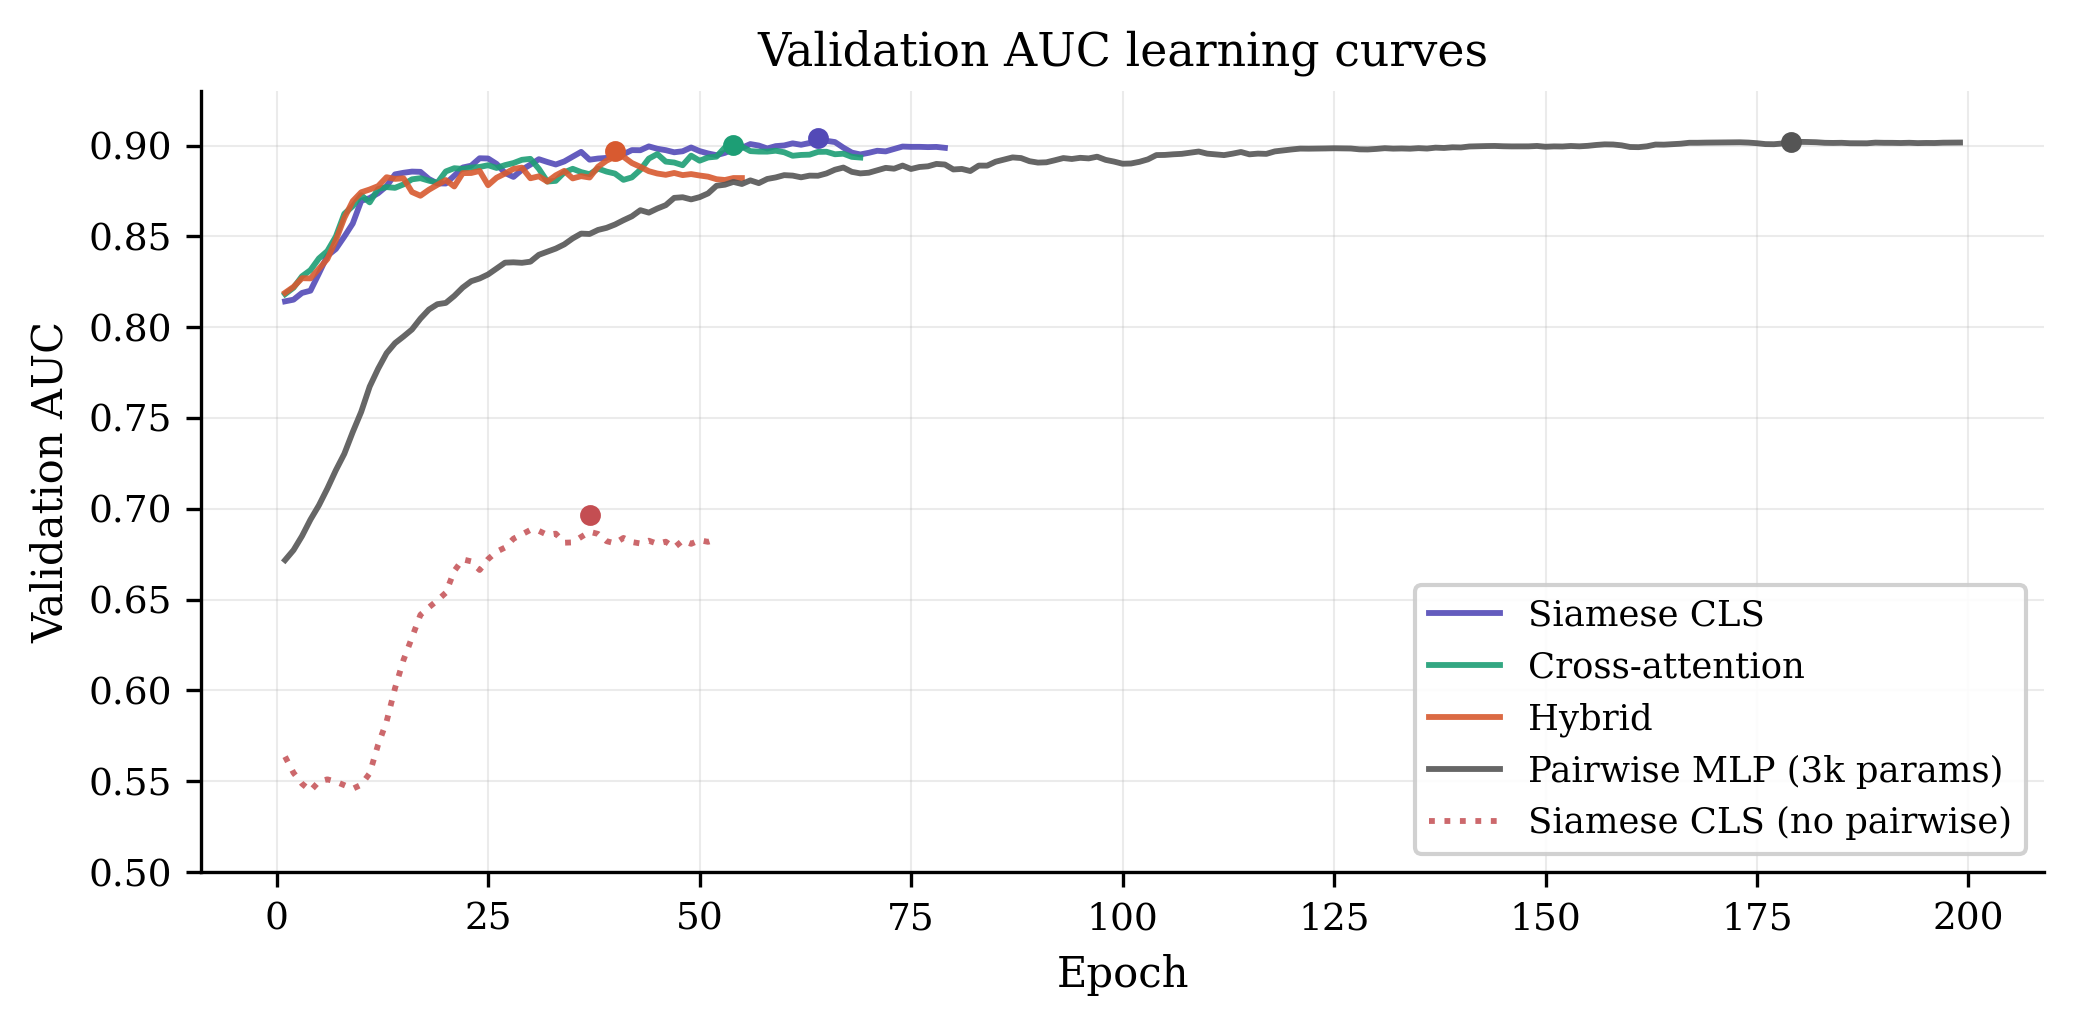
\includegraphics[width=1\textwidth]{figures/val_auc_learning_curves.png}
\caption{Validation AUC learning curves for all transformer architectures and the MLP baseline.}
\label{fig:val_auc_curves}
\end{figure}

All three transformer architectures exhibit a characteristic pattern: the training AUC rises quickly and reaches values above 0.97, while the validation AUC plateaus between 0.88 and 0.90. This gap between training and validation performance is a clear indicator of overfitting that persists despite the use of multiple regularization techniques (dropout, stochastic depth, label smoothing, weight decay, and frame dropout).

\

The Siamese CLS model with $d_{\text{model}}=80$ trains for 79 epochs before early stopping, reaching a training AUC of 0.974 against a best validation AUC of 0.904. The larger $d_{\text{model}}=128$ variant overfits more aggressively: it reaches a training AUC of 0.985 in only 29 epochs while achieving a lower validation AUC of 0.860. The Cross-Attention model trains for 69 epochs with a final training AUC of 0.974 and a best validation AUC of 0.901. The Hybrid model shows a similar pattern, training for 55 epochs to a training AUC of 0.978 and a best validation AUC of 0.897.

\

\begin{figure}[H]
\centering
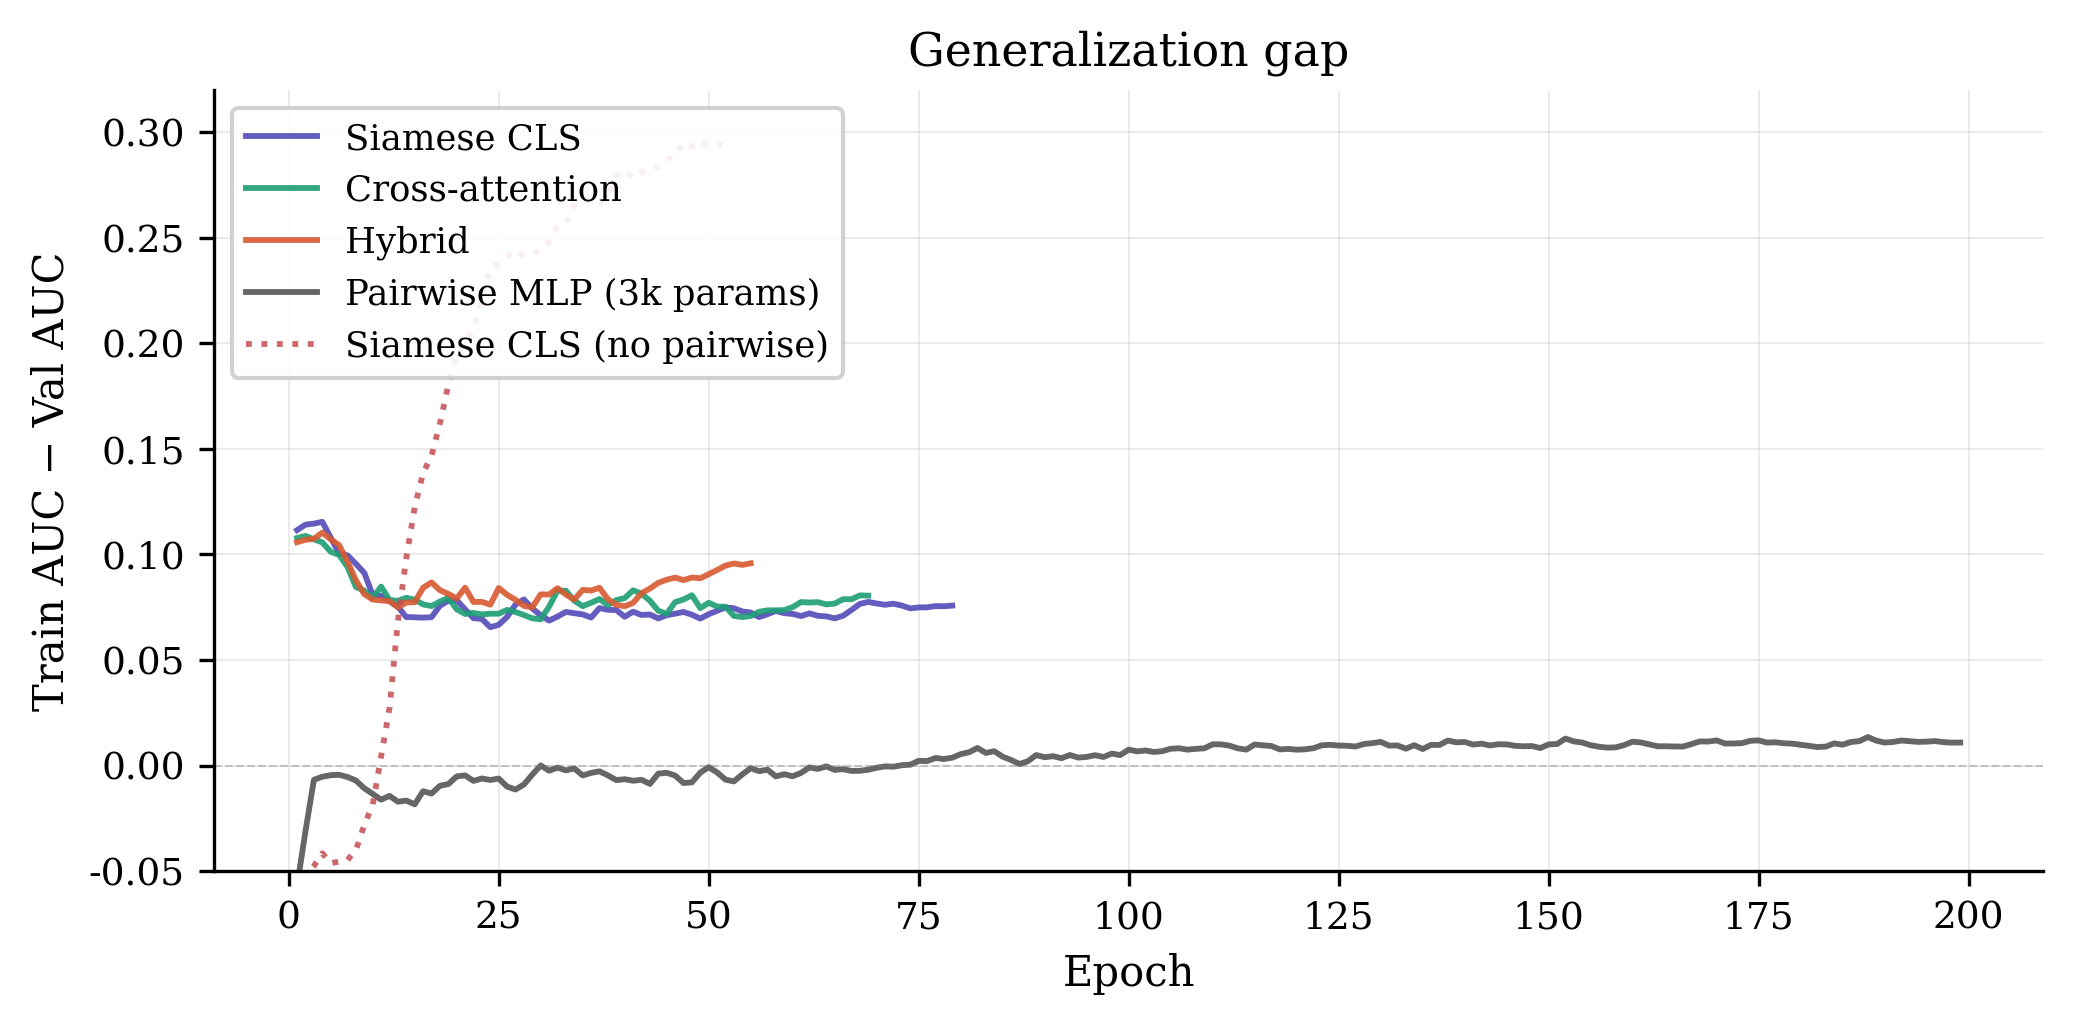
\includegraphics[width=1\textwidth]{figures/generalization_gap.png}
\caption{Generalization gap (train AUC minus validation AUC) across training epochs.}
\label{fig:generalization_gap}
\end{figure}

Figure \ref{fig:generalization_gap} visualizes the generalization gap (train AUC minus validation AUC) across training. All transformer models show a monotonically increasing generalization gap that grows throughout training. The larger Siamese CLS model ($d_{\text{model}}=128$) develops the largest gap, confirming that additional capacity exacerbates overfitting rather than improving generalization.

\

The no pairwise variant reveals an extreme case. During the first 10 epochs, both train and validation AUC remain near 0.50, indicating that the model finds no learnable signal in the raw frame sequences. Between epochs 10 and 20, the training AUC suddenly jumps to 0.85 as the model begins memorizing the training set, while the validation AUC improves only modestly to 0.64. By the end of training, the generalization gap exceeds 0.29 (train AUC 0.977 versus validation AUC 0.682), the largest gap observed across all experiments. This confirms that without pairwise features, the transformer memorizes training pairs through superficial patterns rather than learning generalizable inter-tracklet relationships.

\

The consistent overfitting across all architectures, combined with the observation that larger models overfit more while heavy regularization has limited effect, points to a single root cause: the training set of $\sim$13{,}000 pairs is insufficient for transformer based models. The models have enough capacity to memorize the training data but not enough examples to learn robust decision boundaries.


\subsubsection{Model Size Ablation}\label{sec:size_ablation}
The training inspection reveals that all transformer models overfit the training data. A natural question is whether the bottleneck is model capacity (the models are too small to generalize) or data volume (the models are too large relative to the amount of training data). To answer this question, we conduct a model size ablation study using the Siamese CLS architecture with real+synthetic training data. We vary $d_{\text{model}}$ and $d_{\text{ff}}$ across six configurations while keeping all other hyperparameters fixed, spanning a parameter range from approximately 100k to 2.6M.

\begin{table}[H]
\centering
\begin{tabular}{llcccccc}
\toprule
\textbf{Label} & \textbf{$d_{\text{model}}$} & \textbf{$d_{\text{ff}}$} & \textbf{Params} & \textbf{Test AUC $\uparrow$} & \textbf{Test AP $\uparrow$} & \textbf{Test F1} & \textbf{Best epoch} \\
\midrule
Tiny   & 32  & 64  & $\sim$102k  & \textbf{0.8846} & 0.4795 & 0.4774 & 73 \\
Small  & 48  & 96  & $\sim$173k  & 0.8758 & 0.4880 & 0.4954 & 40 \\
Base   & 80  & 128 & $\sim$343k  & 0.8837 & \textbf{0.5044} & \textbf{0.4987} & 43 \\
Medium & 128 & 256 & $\sim$772k  & 0.8722 & 0.4658 & 0.4701 & 44 \\
Large  & 192 & 384 & $\sim$1.5M  & 0.8633 & 0.4725 & 0.4658 & 27 \\
XLarge & 256 & 512 & $\sim$2.6M  & 0.8754 & 0.4710 & 0.4946 & 42 \\
\bottomrule
\end{tabular}
\caption{Model size ablation for the Siamese CLS architecture with real+synthetic data. All configurations use 4 layers and 4 attention heads (except Tiny which uses 2 heads).}
\label{tab:size_ablation}
\end{table}

The results reveal that performance is remarkably stable across a wide range of model sizes, with no clear benefit from increasing capacity. The Tiny model ($\sim$102k parameters) achieves the highest test AUC of 0.885 despite having the fewest parameters. The Base model ($\sim$343k) follows closely at 0.884, while all larger configurations perform worse: Medium ($\sim$772k) achieves 0.872, Large ($\sim$1.5M) drops to 0.863, and XLarge ($\sim$2.6M) reaches 0.875. No configuration exceeds 0.885, and increasing the parameter count by 25$\times$ (from 102k to 2.6M) provides no improvement.

\

The best epoch column further supports this interpretation. The Tiny model trains for 73 epochs before early stopping, while the Large model triggers early stopping after only 27 epochs. Larger models overfit the training data faster, exhausting the useful signal in fewer iterations and stopping before they can develop robust features. The Tiny model, constrained by its limited capacity, is forced to learn more generalizable patterns from the training data.

\

If larger models achieved higher test performance, the bottleneck would be capacity: the models would need more parameters to represent the decision boundary. Instead, models spanning a 25$\times$ parameter range (102k to 2.6M) all converge to test AUC values between 0.863 and 0.885. This plateau confirms that the performance ceiling is set by the volume and diversity of the training data, not by model capacity.


\subsubsection{MLP Baseline}\label{sec:mlp_baseline}
The model size ablation demonstrates that smaller transformers perform as well as or better than larger ones. Taken to its logical extreme, this raises the question: does the per-frame sequence processing contribute anything at all? To test this, we train a simple multi-layer perceptron (MLP) that operates exclusively on the 12 handcrafted pairwise features, bypassing all per-frame sequence data entirely.

\

The MLP architecture is intentionally minimal: a two-layer feedforward network with hidden dimensions of 64 and 32, layer normalization, GELU activations, and dropout of 0.3. The complete model contains only 3{,}137 trainable parameters. The model receives the same 12 pairwise features that are appended to the transformer classification heads (ReID cosine similarity, SigLIP cosine similarity, temporal gap, spatial distance, jersey agreement, team agreement, and their derived features). Crucially, it does not have access to any per-frame information, raw embeddings, or sequence data.

\begin{table}[H]
\centering
\begin{tabular}{lcccc}
\toprule
\textbf{Model} & \textbf{Params} & \textbf{Test AUC $\uparrow$} & \textbf{Test AP $\uparrow$} & \textbf{Test F1} \\
\midrule
Pairwise MLP            & 3{,}137    & \textbf{0.885} & \textbf{0.494} & 0.491 \\
\midrule
Siamese CLS (best)      & 299{,}000  & 0.886 & 0.494 & \textbf{0.497} \\
Cross-Attention (best)   & 252{,}000  & 0.882 & 0.475 & 0.471 \\
Hybrid (best)            & 302{,}000  & 0.875 & 0.474 & 0.466 \\
\bottomrule
\end{tabular}
\caption{Pairwise MLP compared against all transformer architectures. The MLP uses only 12 pairwise features and no sequence data.}
\label{tab:mlp_comparison}
\end{table}

The results in Table \ref{tab:mlp_comparison} are striking. The pairwise MLP with 3{,}137 parameters achieves a test AUC of 0.885 and an average precision of 0.494, matching the best transformer (Siamese CLS: 0.886 AUC, 0.494 AP) within measurement noise. The MLP outperforms both the Cross-Attention and Hybrid architectures despite having roughly 80$\times$ fewer parameters and no access to per-frame data.

\

The MLP training dynamics also differ substantially from the transformers. The MLP trains for 199 epochs (compared to 55 to 79 for the transformers), and its generalization gap remains much smaller: the final training AUC is 0.913 versus a validation AUC of 0.902, a gap of only 0.011. In contrast, the best transformer achieves a training AUC of 0.974 against a validation AUC of 0.904, a gap of 0.070. The MLP's smaller capacity prevents it from memorizing the training data, forcing it to learn more general patterns from the pairwise features.

\

Note that the MLP was trained on the real only data (4{,}403 pairs) rather than the real+synthetic data (13{,}212 pairs), yet it still matches the transformers trained on the larger dataset. This further underscores the efficiency of the pairwise feature representation: the 12 handcrafted features already capture the relevant inter-tracklet relationships so effectively that a minimal model can exploit them with less data.

\

This result carries an important implication. The per-frame sequence data that the transformers process through hundreds of thousands of parameters, including 512 dimensional ReID embeddings, 768 dimensional SigLIP embeddings, bounding box features, and jersey and team predictions per frame, provides no measurable advantage over the aggregated pairwise features. The transformers are unable to extract additional useful information from the raw sequences beyond what is already captured by the handcrafted pairwise comparisons. With approximately 13{,}000 training pairs, the task does not provide enough examples for transformers to learn frame level matching patterns that outperform simple aggregated statistics.


\subsubsection{Takeaway}\label{sec:transformer_takeaway}
The transformer experiments reveal a consistent finding across all experiments: the available training data is insufficient for transformer based models to outperform simpler approaches on the tracklet merging task. Several complementary pieces of evidence support this conclusion.

\

First, removing pairwise features (Section \ref{sec:pairwise_ablation}) causes the transformer to fail almost completely, demonstrating that self-attention cannot learn inter-tracklet relationships from raw frame sequences with the available data. Second, the training inspection (Section \ref{sec:training_inspection}) shows that all transformers overfit severely, with training AUC exceeding 0.97 while validation AUC plateaus around 0.90, despite extensive regularization. Third, the model size ablation (Section \ref{sec:size_ablation}) confirms that the bottleneck is data volume rather than model capacity, as models spanning a 7.5$\times$ parameter range all plateau at similar test AUC while larger models overfit faster. Finally, the MLP baseline (Section \ref{sec:mlp_baseline}) provides the strongest evidence: a 3{,}137 parameter model operating on 12 handcrafted features matches the best transformer with 299{,}000 parameters and full sequence access.

\

These results suggest that transformers are not the right tool for this problem at this data scale. The SoccerNet Player-Tracking dataset contains only 57 training sequences, yielding approximately 4{,}000 real positive pairs. Even with synthetic augmentation tripling the dataset to 13{,}000 pairs, transformers cannot learn to exploit per-frame patterns beyond what aggregated statistics already capture. The Cross-Attention architecture, which enables direct frame level comparison, and the Hybrid model, which enriches frame representations before comparison, both fail to leverage their architectural advantages.

\

This does not imply that transformers are fundamentally unsuited for tracklet merging. With significantly more training data (potentially from larger tracking datasets or domain transfer), the per-frame sequence processing could provide an advantage by capturing temporal appearance patterns, detecting occlusion events, or learning frame importance weighting that aggregated features cannot express. The architecture is sound; the data is the limiting factor. For the current dataset and task, the XGBoost connector trained on 47 handcrafted features remains the more practical and effective approach. The end-to-end comparison of all connectors through the complete pipeline is presented in Section \ref{sec:connector_comparison}.
